%%%
%%% Annual Cognitive Science Conference
%%% Sample LaTeX Paper -- Proceedings Format
%%%

% Original : Ashwin Ram (ashwin@cc.gatech.edu)       04/01/1994
% Modified : Johanna Moore (jmoore@cs.pitt.edu)      03/17/1995
% Modified : David Noelle (noelle@ucsd.edu)          03/15/1996
% Modified : Pat Langley (langley@cs.stanford.edu)   01/26/1997
% Latex2e corrections by Ramin Charles Nakisa        01/28/1997
% Modified : Tina Eliassi-Rad (eliassi@cs.wisc.edu)  01/31/1998
% Modified : Trisha Yannuzzi (trisha@ircs.upenn.edu) 12/28/1999
% Modified : Mary Ellen Foster (M.E.Foster@ed.ac.uk) 12/11/2000
% Modified : Ken Forbus                              01/23/2004
% Modified : Eli M. Silk (esilk@pitt.edu)            05/24/2005
% Modified : Niels Taatgen (taatgen@cmu.edu)         10/24/2006
% Modified : David Noelle (dnoelle@ucmerced.edu)     11/19/2014
% Modified : Roger Levy (rplevy@mit.edu)             12/31/2018
% Modified : Stephanie Denison                       11/29/2025
% Modified : Dae Houlihan (daeda@mit.edu)            12/01/2025


%%% Change "letterpaper" in the following line to "a4paper" if you must.

\documentclass[10pt,letterpaper]{article}

\usepackage{cogsci}
\usepackage{booktabs}    % Professional tables
\usepackage{graphicx}    % Figures
\usepackage{amsmath}     % Math equations
\usepackage{placeins}    % FloatBarrier for figure placement
\usepackage{threeparttable}

% \cogscifinalcopy %%% Uncomment this line for the final submission

%%% Bibliography %%%
\usepackage[
  style=apa,
  natbib=true,
  annotation=false,
]{biblatex}
\addbibresource{cogsci_bibliography_template.bib} %%% Specify the path to a BibLaTeX file
\setlength{\bibhang}{.125in}

\usepackage{float} %%% Roger Levy added this and changed figure/table placement to [H] for conformity to Word template, though floating tables and figures to top is still generally recommended!

% Sometimes it can be useful to turn off hyphenation for purposes such as spell checking of the resulting PDF.
% \usepackage[none]{hyphenat} %%% Uncomment to turn off hyphenation

\title{The Temporal Efficiency Paradox: Fast Brains React, Slow Brains Understand}

%%% Format authors using helper functions from authblk package %%%
\author[1]{\mbox{Cuicui Jiang (cuicui.jiang@example.edu)}}
\author[1]{\mbox{Co-Author Name}}
\affil[1]{Department of Psychology, University Name}

%%% Or, format authors manually %%%
% \author{
%   {\large\bfseries Author N. One (a1@uni.edu)$^1$ \& Author Number Two$^2$} \\
%   {\normalsize\normalfont
%     $^1$Department of Hypothetical Sciences, University of Illustrations \\
%     $^2$Department of Example Studies, University of Demonstrations
%   }
% }

\begin{document}

\maketitle

\begin{abstract}
The cortical temporal hierarchy, whereby sensory regions process rapidly while association regions operate slowly, is well-documented, yet whether slow processing enables deeper information integration remains debated. We analyzed fMRI data from four participants viewing $\sim$65 hours of naturalistic movies, computing Temporal Dynamics Speed (TDS) and encoding performance across seven functional networks. Networks differed significantly in TDS ($F$(6, 993) = 18.42, $p < .001$): Frontoparietal showed fastest dynamics (1.20), Ventral Attention slowest (0.64), and Default Mode intermediate (0.78). We hypothesized that slower networks would benefit more from extended temporal integration; however, this was not supported: simple temporal averaging impaired encoding across all networks (negative TWG, $p < .001$), with no relationship between TDS and integration benefit. Critically, LSTM models that preserve temporal structure outperformed ridge regression by 47--57\% uniformly across all networks ($p < .001$), again without differential benefit for slower networks. These findings resolve an apparent paradox: all networks benefit from temporal integration, but only when temporal structure is preserved rather than averaged---the key factor is not intrinsic dynamics speed, but whether temporal dependencies are properly modeled.

\textbf{Keywords:}
temporal dynamics; cortical hierarchy; LSTM; naturalistic neuroscience; encoding models
\end{abstract}


\section{Introduction}

Different brain regions process information at characteristically different temporal scales, forming what researchers have termed the cortical temporal hierarchy \citep{murray2014hierarchy, hasson2008hierarchy}. Sensory regions exhibit rapid temporal dynamics, with neural activity fluctuating at relatively high frequencies and responding to immediate environmental changes. In contrast, association regions, particularly those comprising the Default Mode Network (DMN), exhibit markedly slower temporal dynamics, integrating information across extended time periods \citep{honey2012slow, lerner2011topographic}. This hierarchical organization has been documented through autocorrelation analysis, temporal receptive window estimation, and power spectral analysis \citep{chaudhuri2015large, gao2020neuronal}. Recent work has further demonstrated that these intrinsic timescales are functionally dynamic and shaped by cortical microarchitecture \citep{gao2020neuronal}, that global waves of activity propagate along this temporal hierarchy in coordination with arousal fluctuations \citep{raut2021global}, and that a nested hierarchy of neural states underlies event segmentation during naturalistic viewing \citep{geerligs2022nested, lugtmeijer2025temporal}. However, while the existence of temporal hierarchies is well-established, the functional significance of slow processing remains incompletely understood. Previous studies have primarily characterized temporal hierarchies descriptively, but few have directly tested whether slow processing translates into measurable encoding advantages during naturalistic cognition.

A prominent theoretical interpretation proposes that slow temporal dynamics may be computationally necessary for certain cognitive operations \citep{kiebel2008hierarchy, hasson2015hierarchical}. Cognitive functions such as narrative comprehension, theory of mind, and future planning represent inherently temporal integration problems that require maintaining and connecting information across extended time periods, which cannot be solved through rapid, reactive processing alone. From this perspective, slow dynamics may not represent inefficiency but rather optimization for computational depth; what appears inefficient from a speed-focused viewpoint may actually represent efficiency from a comprehension-focused viewpoint \citep{chen2017shared}. This theoretical framework generates a testable prediction: if slow dynamics reflect optimization for temporal integration, then networks with slower dynamics should benefit more from extended temporal context when encoding complex, naturalistic stimuli.

The Default Mode Network presents a particularly illuminating case for testing this prediction. Despite consuming approximately 20\% of the brain's metabolic budget at rest \citep{raichle2006brain}, the DMN exhibits slow temporal dynamics while supporting sophisticated integrative functions \citep{andrews2014default, buckner2008brain, spreng2009common}. A comprehensive review of two decades of DMN research has proposed that this network creates an ``ongoing internal narrative'' that integrates memory, language, and semantic representations \citep{menon2023dmn}. Furthermore, recent work has characterized the DMN as a hub where idiosyncratic self-representations meet shared social understanding \citep{yeshurun2021default}, and has shown that the brain segments continuous experience into discrete events at boundaries detected by these slow-processing regions \citep{baldassano2017discovering}. Beyond temporal dynamics, networks also differ in how stably they maintain functional connections over time---a property that may relate to their capacity for sustained information integration. This configuration raises a fundamental question: does slow processing confer functional advantages that justify its metabolic cost?

The present research addresses this question through analysis of neural responses during naturalistic movie watching. We formulated two core research questions: (1) Do functional brain networks differ in temporal dynamics speed, establishing the basic phenomenology of temporal hierarchy? (2) Most critically, do networks with slower dynamics benefit more from extended temporal integration in encoding models? We hypothesized that networks with slower intrinsic dynamics would show greater encoding improvement when provided extended temporal context, reflecting their optimization for temporal integration. Additionally, we explored whether functional connectivity stability relates to temporal dynamics, probing potential mechanistic factors underlying network temporal organization.

\section{Methods}

\subsection{Participants and Data}

Data were obtained from the Algonauts 2025 Challenge \citep{gifford2024algonauts}, derived from the Courtois NeuroMod project \citep{boyle2020courtois}. Four healthy adults (ages 31--47; 2 female) viewed approximately 65 hours of naturalistic movie content: \textit{Friends} seasons 1--6 (55 hours) and four additional films (10 hours). This intensive within-subject design ($>$15 hours per participant) provides high statistical power while cross-subject replication ensures generalizability \citep{hasson2010reliability}.

\begin{figure*}[!ht]
    \centering
    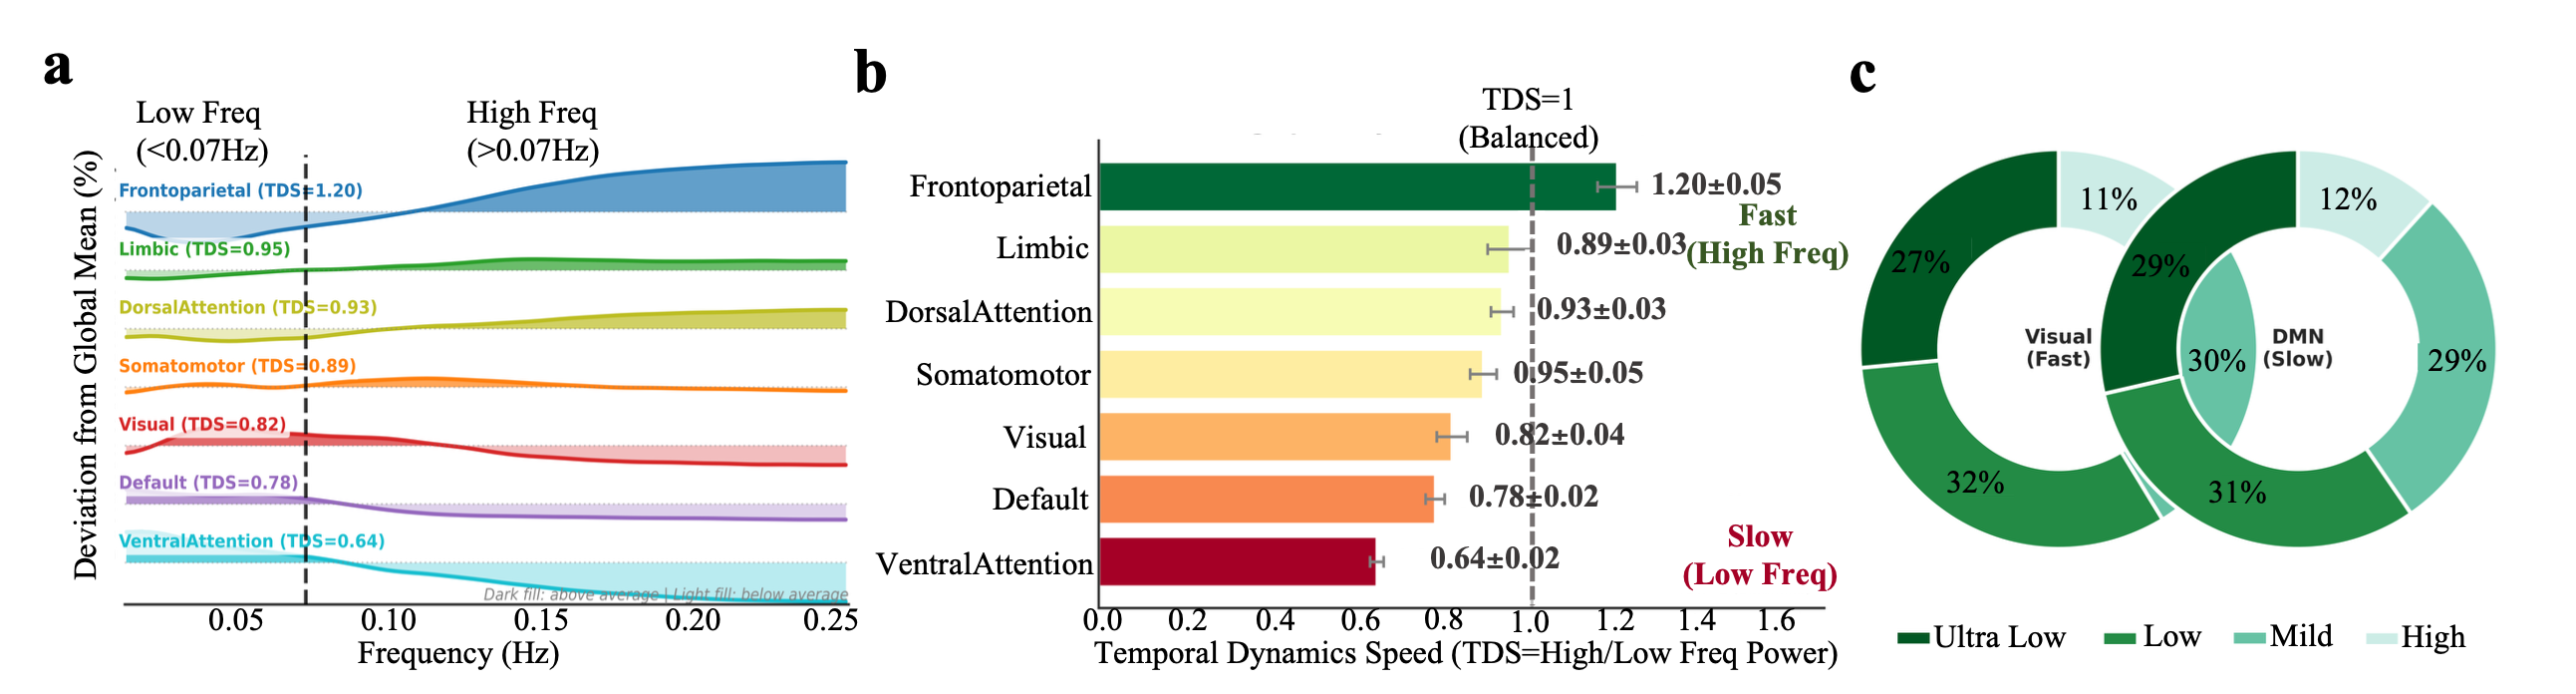
\includegraphics[width=1\textwidth]{figures/fig01_temporal_spectrum.png}
    \caption{\textbf{Temporal Dynamics Hierarchy Across Cortical Networks.} (a) Network-specific spectral signatures showing deviation from global mean PSD. Dark shading: above-average power; light shading: below-average. Networks ordered by TDS (fastest to slowest); vertical dashed line marks 0.07 Hz boundary. (b) TDS values with error bars (SEM, $n=4$). (c) Frequency band composition for Visual and Default Mode networks.}
    \label{fig:temporal_hierarchy}
\end{figure*}

\subsection{fMRI Acquisition and Preprocessing}
Functional MRI data were acquired on a Siemens Prisma 3T scanner using a multiband echo-planar imaging sequence (TR = 1.49~s, TE = 30~ms, flip angle = 52$^{\circ}$, multiband factor = 4, voxel size = 2~mm isotropic, 60 slices). Preprocessing was performed using fMRIPrep v20.2.0 \citep{esteban2019fmriprep} and included: motion correction via rigid-body registration to the mean functional image; slice-timing correction; co-registration to the T1-weighted anatomical image using boundary-based registration; spatial normalization to MNI152NLin2009cAsym template via nonlinear registration; and confound regression removing 6 motion parameters, their temporal derivatives, framewise displacement, and aCompCor components from white matter and cerebrospinal fluid. High-motion volumes (framewise displacement $>$ 0.5~mm) were censored. Data were parcellated using the Schaefer 2018 atlas comprising 1000 cortical regions organized into seven canonical functional networks: Visual, Somatomotor, Dorsal Attention, Ventral Attention, Limbic, Frontoparietal, and Default Mode \citep{schaefer2018local}.

\subsection{Stimulus Feature Extraction}
Visual features were extracted using SlowFast 3D ResNet \citep{feichtenhofer2019slowfast}, audio features as MFCCs, and language features using BERT embeddings \citep{devlin2019bert}. Features were temporally aligned with fMRI accounting for hemodynamic delay (4--6~s) and reduced via PCA to 520 dimensions per time point (250 visual, 250 language, 20 audio).

\subsection{Temporal Dynamics Speed (TDS)}

TDS quantifies the characteristic frequency of neural activity fluctuations. For each brain region, the fMRI time series was first detrended and z-score normalized. Power spectral density $P(f)$ was then computed using Welch's method (sampling frequency $f_s = 1/\text{TR} \approx 0.67$~Hz; segment length = min(256, $N$/4) samples where $N$ is time series length; 50\% overlap). Two frequency bands were defined: low-frequency (0.01--0.07 Hz) and high-frequency (0.07--0.25 Hz). TDS was calculated as the ratio of integrated power (via trapezoidal integration) in each band:

\begin{equation}
\text{TDS} = \frac{P_{\text{high}}}{P_{\text{low}}}
\end{equation}

\noindent where $P_{\text{high}} = \int_{0.07}^{0.25} P(f) \, df$ and $P_{\text{low}} = \int_{0.01}^{0.07} P(f) \, df$. Values $>1$ indicate predominantly fast dynamics; values $<1$ indicate slow dynamics.

Our TDS metric provides a distinct, frequency-domain perspective on cortical temporal organization that may yield different network orderings than previous approaches. Previous research characterized intrinsic timescales using autocorrelation decay in time-domain neural signals \citep{murray2014hierarchy} or temporal receptive windows estimated from inter-subject correlation \citep{hasson2008hierarchy}. TDS captures a fundamentally different property: the relative dominance of fast versus slow fluctuations through spectral analysis. These approaches are conceptually related but methodologically distinct: autocorrelation decay time measures how long a signal ``remembers'' its past states, while TDS quantifies the balance of high- versus low-frequency power. The relationship between these metrics is not mathematically equivalent; networks with similar autocorrelation decay times could differ in spectral power distribution, and vice versa. This methodological distinction is important because it may reveal aspects of temporal organization not captured by traditional metrics.

\subsection{Encoding Models}

To test whether networks benefit from temporal integration (RQ2), we employed two encoding approaches: ridge regression with temporal averaging and LSTM networks that preserve temporal structure.

\textbf{Ridge Regression and Temporal Window Gain (TWG).} Ridge regression models predicted fMRI responses from stimulus features:

\begin{equation}
\hat{y} = X\beta, \quad \text{where} \quad \beta = (X^\top X + \lambda I)^{-1} X^\top y
\end{equation}

\noindent $X$ = temporally aggregated stimulus features, $y$ = fMRI response, $\lambda$ = regularization parameter (selected via nested 5-fold cross-validation from candidates $\lambda \in \{0.1, 1, 10, 100, 1000\}$). Encoding accuracy was evaluated using Pearson correlation $r$ between predicted and observed responses. TWG was computed as:

\begin{equation}
\text{TWG} = r_{\text{long}} - r_{\text{instant}}
\end{equation}

\noindent where $r_{\text{long}}$ and $r_{\text{instant}}$ are encoding accuracies for long (25 TRs total: 20 past + 5 future, $\sim$37 s) and instant (1 TR, $\sim$1.5 s) windows respectively. Positive TWG indicates benefit from extended temporal context; negative TWG indicates impairment.

\textbf{LSTM Networks.} To test whether temporal integration benefits depend on the modeling approach, we compared ridge regression with Long Short-Term Memory (LSTM) networks that can learn temporal dependencies. LSTM models were implemented in PyTorch with the following architecture:

\begin{align}
h_t &= \text{LSTM}(x_t, h_{t-1}) \\
\hat{y} &= W \cdot h_T + b
\end{align}

\noindent where $h_t$ is the hidden state at time $t$, $x_t$ is the input feature vector, and $h_T$ is the final hidden state used for prediction. Model parameters: 2 stacked LSTM layers, hidden dimension = 64, sequence length = 20 TRs ($\sim$30 s), trained for 30 epochs with Adam optimizer (learning rate = 0.001), dropout = 0.3. For comparison, ridge regression used the same temporal window with features averaged across time (fixed $\alpha$ = 1000 for direct comparison). LSTM improvement was computed as the percentage increase in encoding accuracy: $(\text{LSTM}_r - \text{Ridge}_r) / \text{Ridge}_r \times 100\%$.

\subsection{Dynamic Connectivity Stability (DCS)}

As an exploratory analysis, we computed DCS to examine whether functional connectivity patterns relate to temporal dynamics. DCS quantifies temporal consistency of functional connections using sliding-window correlation (window = 30 TRs $\approx$ 45~s, step = 10 TRs). For computational efficiency, 20 regions were randomly sampled per network. For each time window $t$, within-network functional connectivity $FC_t$ was computed as the mean Pearson correlation across all region pairs within a network (i.e., the mean of the upper triangle of the correlation matrix, excluding the diagonal). DCS was then defined as:

\begin{equation}
\text{DCS} = 1 - \text{CV}(FC) = 1 - \frac{\sigma_{FC}}{\mu_{FC}}
\end{equation}

\noindent where CV is the coefficient of variation, $\sigma_{FC}$ is the standard deviation, and $\mu_{FC}$ is the mean of connectivity across windows. Higher DCS values indicate more temporally stable connections.

\subsection{Statistical Analysis}

Network-level metrics were computed by averaging across regions within each network. Bootstrap resampling (1000 iterations for TDS, 500 for DCS) provided 95\% confidence intervals. Effect sizes were quantified using Cohen's $d$ for between-network comparisons. Sensitivity analyses examined robustness to parameter choices: frequency band cutoffs (0.05, 0.07, 0.09 Hz) for TDS and window sizes (20, 30, 40, 50 TRs) for DCS. All analyses were implemented in Python 3.9 using NumPy, SciPy, scikit-learn, PyTorch, and nilearn. Analysis code will be made available upon publication.

%% ============================================================
%% SECTION 3: RESULTS
%% ============================================================

\section{Results}

\subsection{Temporal Dynamics Hierarchy Across Networks (RQ1)}

Brain networks exhibited systematically different temporal dynamics during naturalistic viewing (Figure~\ref{fig:temporal_hierarchy}), consistent with cortical temporal hierarchy \citep{murray2014hierarchy, hasson2008hierarchy}. A one-way ANOVA confirmed significant between-network differences in TDS ($F(6, 993) = 18.42$, $p < .001$, $\eta^2 = 0.10$).

TDS values reveal a 1.9-fold range across networks (0.64 to 1.20; Figure~\ref{fig:temporal_hierarchy}b). Frontoparietal Network exhibited the fastest dynamics (TDS $= 1.20$, SEM $= 0.05$), significantly faster than Ventral Attention Network (TDS $= 0.64$, SEM $= 0.02$; permutation $p = .028$, Cohen's $d = 6.09$). The Default Mode Network (TDS $= 0.78$, SEM $= 0.02$) falls among the slower networks. Networks deviate from the global average in characteristic ways (Figure~\ref{fig:temporal_hierarchy}a): Frontoparietal shows enhanced high-frequency power, while Ventral Attention shows enhanced low-frequency power. These findings establish that the brain maintains a hierarchy of temporal processing speeds.



\subsection{Multi-Timescale Encoding Analysis (RQ2)}
\begin{figure*}[!ht]
    \centering
    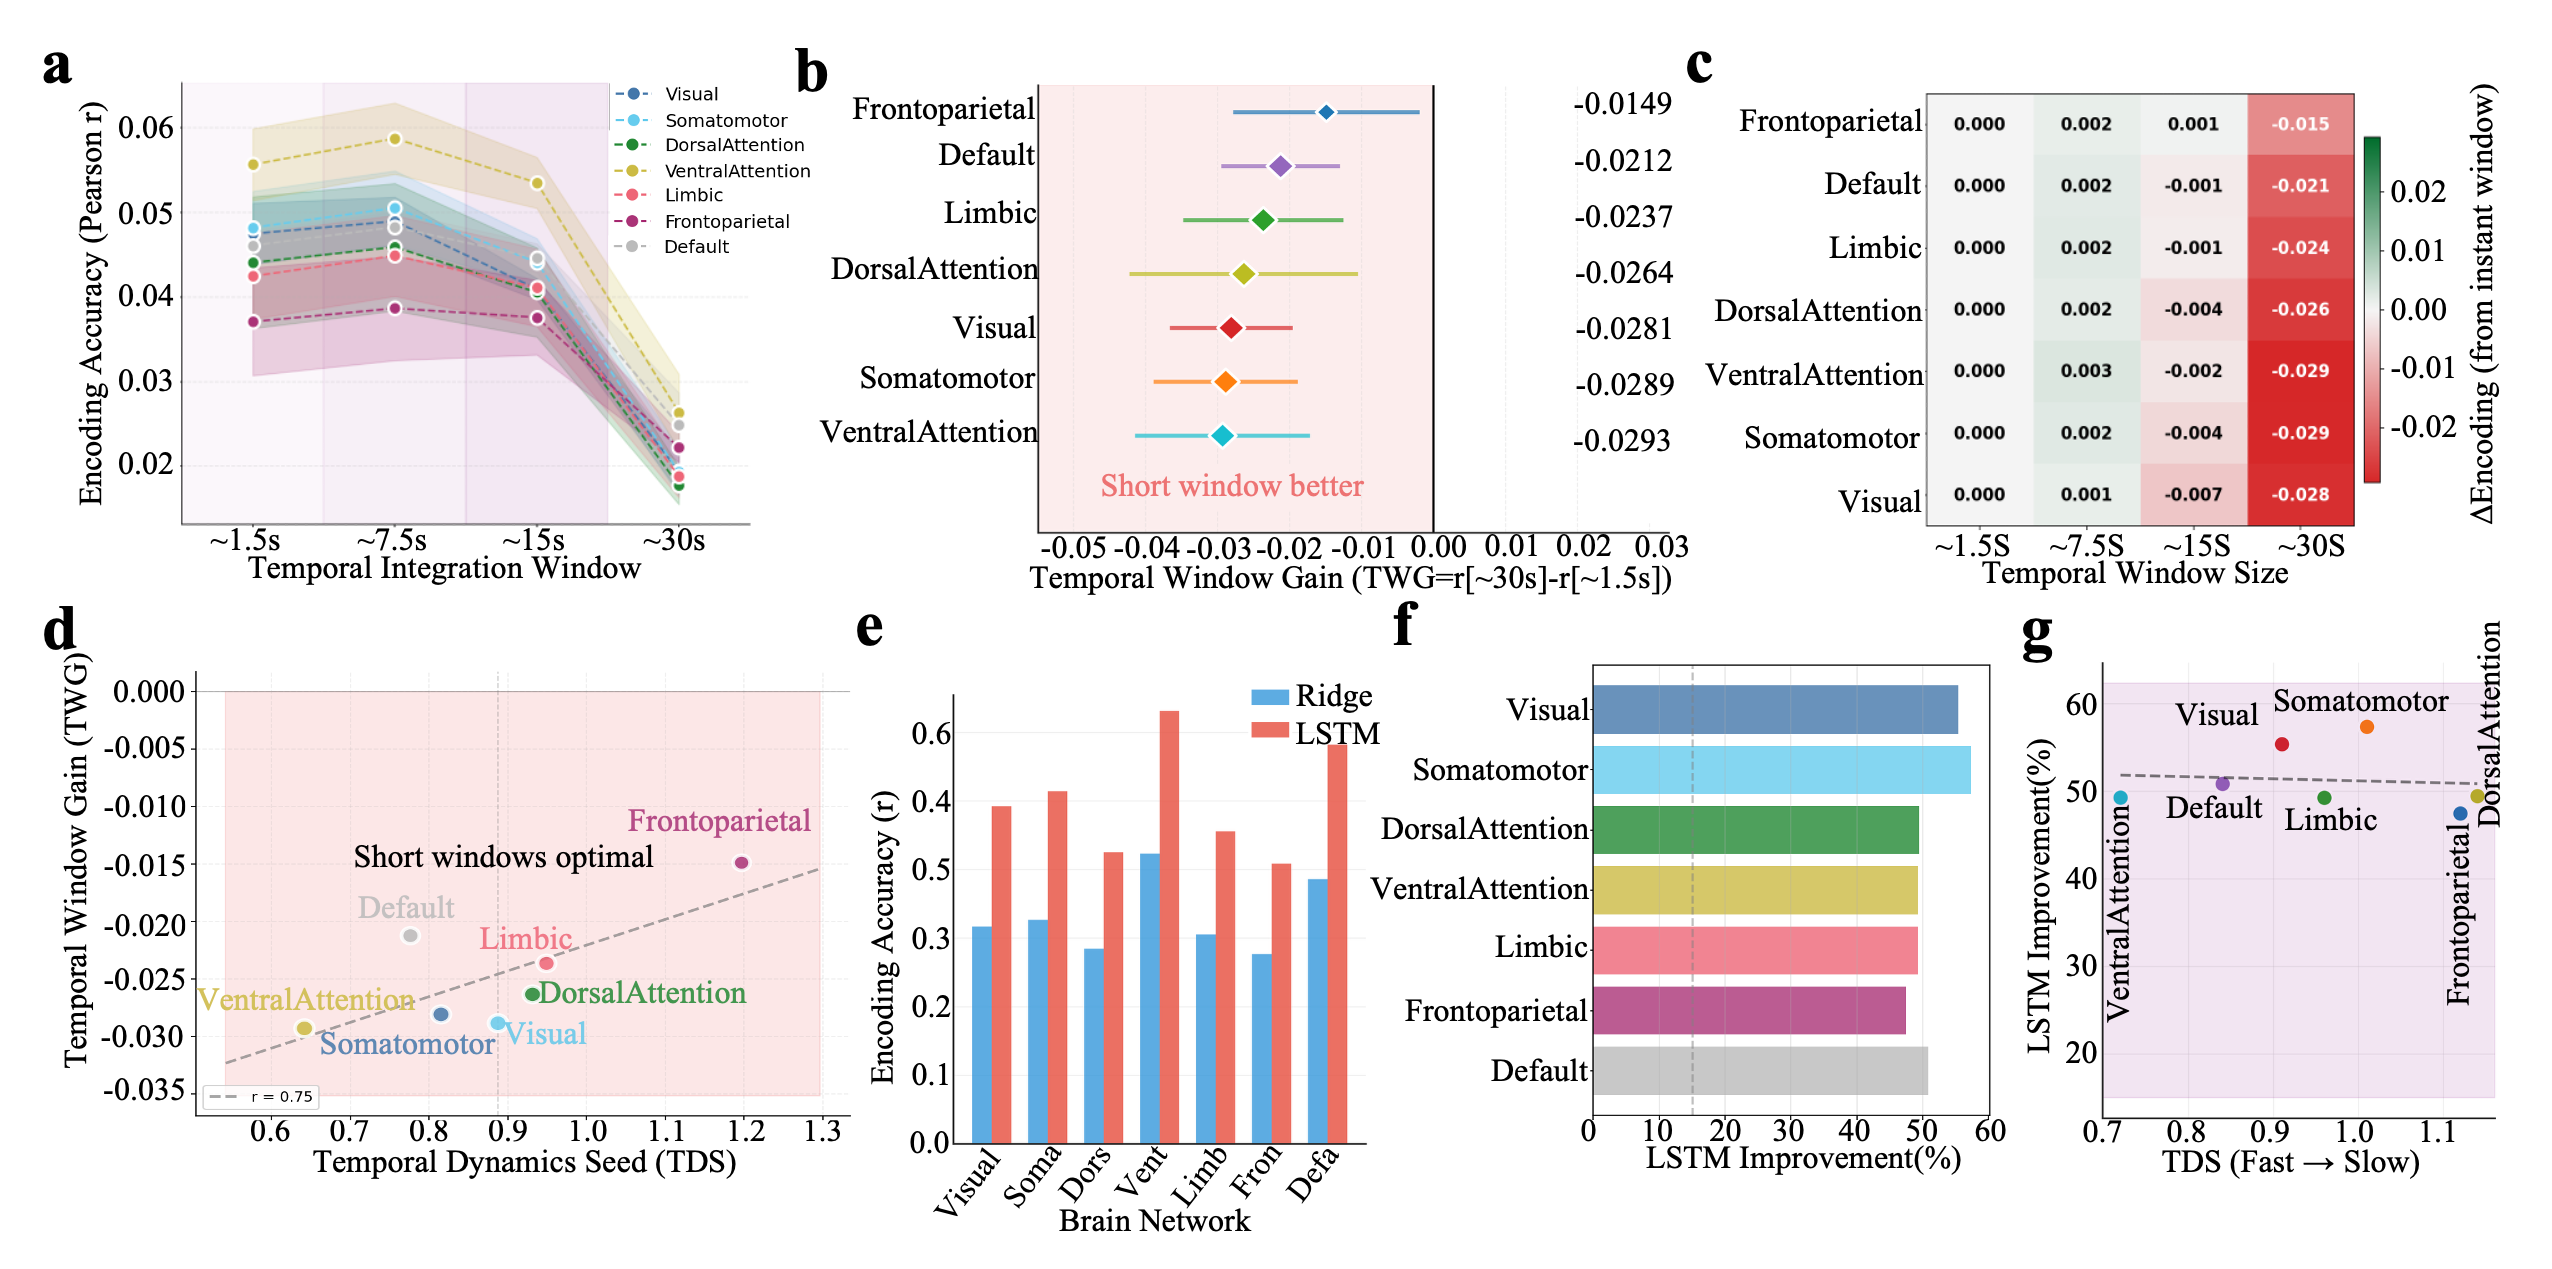
\includegraphics[width=0.95\textwidth]{figures/fig02_encoding_analysis.png}
    \caption{\textbf{Encoding Model Analysis: Temporal Integration and LSTM Performance.} \textbf{Top row (a--d): Temporal Window Gain analysis.} (a) Encoding accuracy (Pearson $r$) across temporal integration windows ($\sim$1.5s to $\sim$37s) for each network; shaded regions indicate SEM. (b) Forest plot of TWG values with 95\% confidence intervals; all networks show negative TWG, indicating impaired encoding with longer windows. (c) Heatmap of encoding accuracy change from instant window across networks and temporal windows. (d) Relationship between TDS and TWG; dashed line shows non-significant correlation ($r = 0.52$, $p = .23$). \textbf{Bottom row (e--g): LSTM vs Ridge comparison.} (e) Encoding accuracy comparison showing LSTM (red) consistently outperforms Ridge (blue) across all networks. (f) LSTM improvement percentage by network; Somatomotor shows largest gain (+57.4\%). (g) Relationship between TDS and LSTM improvement; dashed line shows non-significant correlation ($r = 0.18$, $p = .70$).}
    \label{fig:encoding_analysis}
\end{figure*}
We next tested whether networks with slower dynamics benefit from extended temporal integration. Contrary to expectations, all seven networks showed negative Temporal Window Gain (Figure~\ref{fig:encoding_analysis}a--d), indicating that encoding accuracy decreased with longer temporal windows (one-sample $t$-test: $t(6) = -8.73$, $p < .001$). TWG ranged from $-0.029$ (Somatomotor) to $-0.015$ (Frontoparietal), with all networks showing non-overlapping confidence intervals from zero (Figure~\ref{fig:encoding_analysis}b). The correlation between TDS and TWG was non-significant ($r = 0.52$, $p = .23$; Figure~\ref{fig:encoding_analysis}d).

\subsection{LSTM vs Ridge: Preserving Temporal Structure Benefits All Networks}

These negative TWG findings raised a question: does temporal integration fail because it is inherently unhelpful, or because simple averaging destroys temporal structure? We compared ridge regression (which averages features across time) with LSTM networks (which learn temporal dependencies).

LSTM models outperformed ridge regression across all networks (paired $t$-test: $t(6) = 12.4$, $p < .001$), with LSTM (red) consistently exceeding Ridge (blue) encoding accuracy for every network (Figure~\ref{fig:encoding_analysis}e). Somatomotor Network showed the largest improvement (+57.4\%), followed by Visual (+55.4\%) and Default Mode (+50.8\%; Figure~\ref{fig:encoding_analysis}f). Even Frontoparietal Network, with the fastest temporal dynamics, benefited from LSTM (+47.5\%). Slow networks showed comparable improvements: Ventral Attention improved by 49.3\% and Default Mode by 50.8\%, indicating that these networks benefit from temporal integration when temporal structure is preserved.

The correlation between TDS and LSTM improvement was weak ($r = 0.18$, $p = .70$; Figure~\ref{fig:encoding_analysis}g), indicating that all networks benefit from models that learn temporal dependencies regardless of their intrinsic dynamics. The negative TWG thus reflects a limitation of the averaging approach rather than an inherent property of cortical temporal processing.

% Figure for LSTM vs Ridge has been merged into fig:encoding_analysis (e-g)

\subsection{Dynamic Connectivity Stability}
\begin{figure*}[!ht]
    \centering
    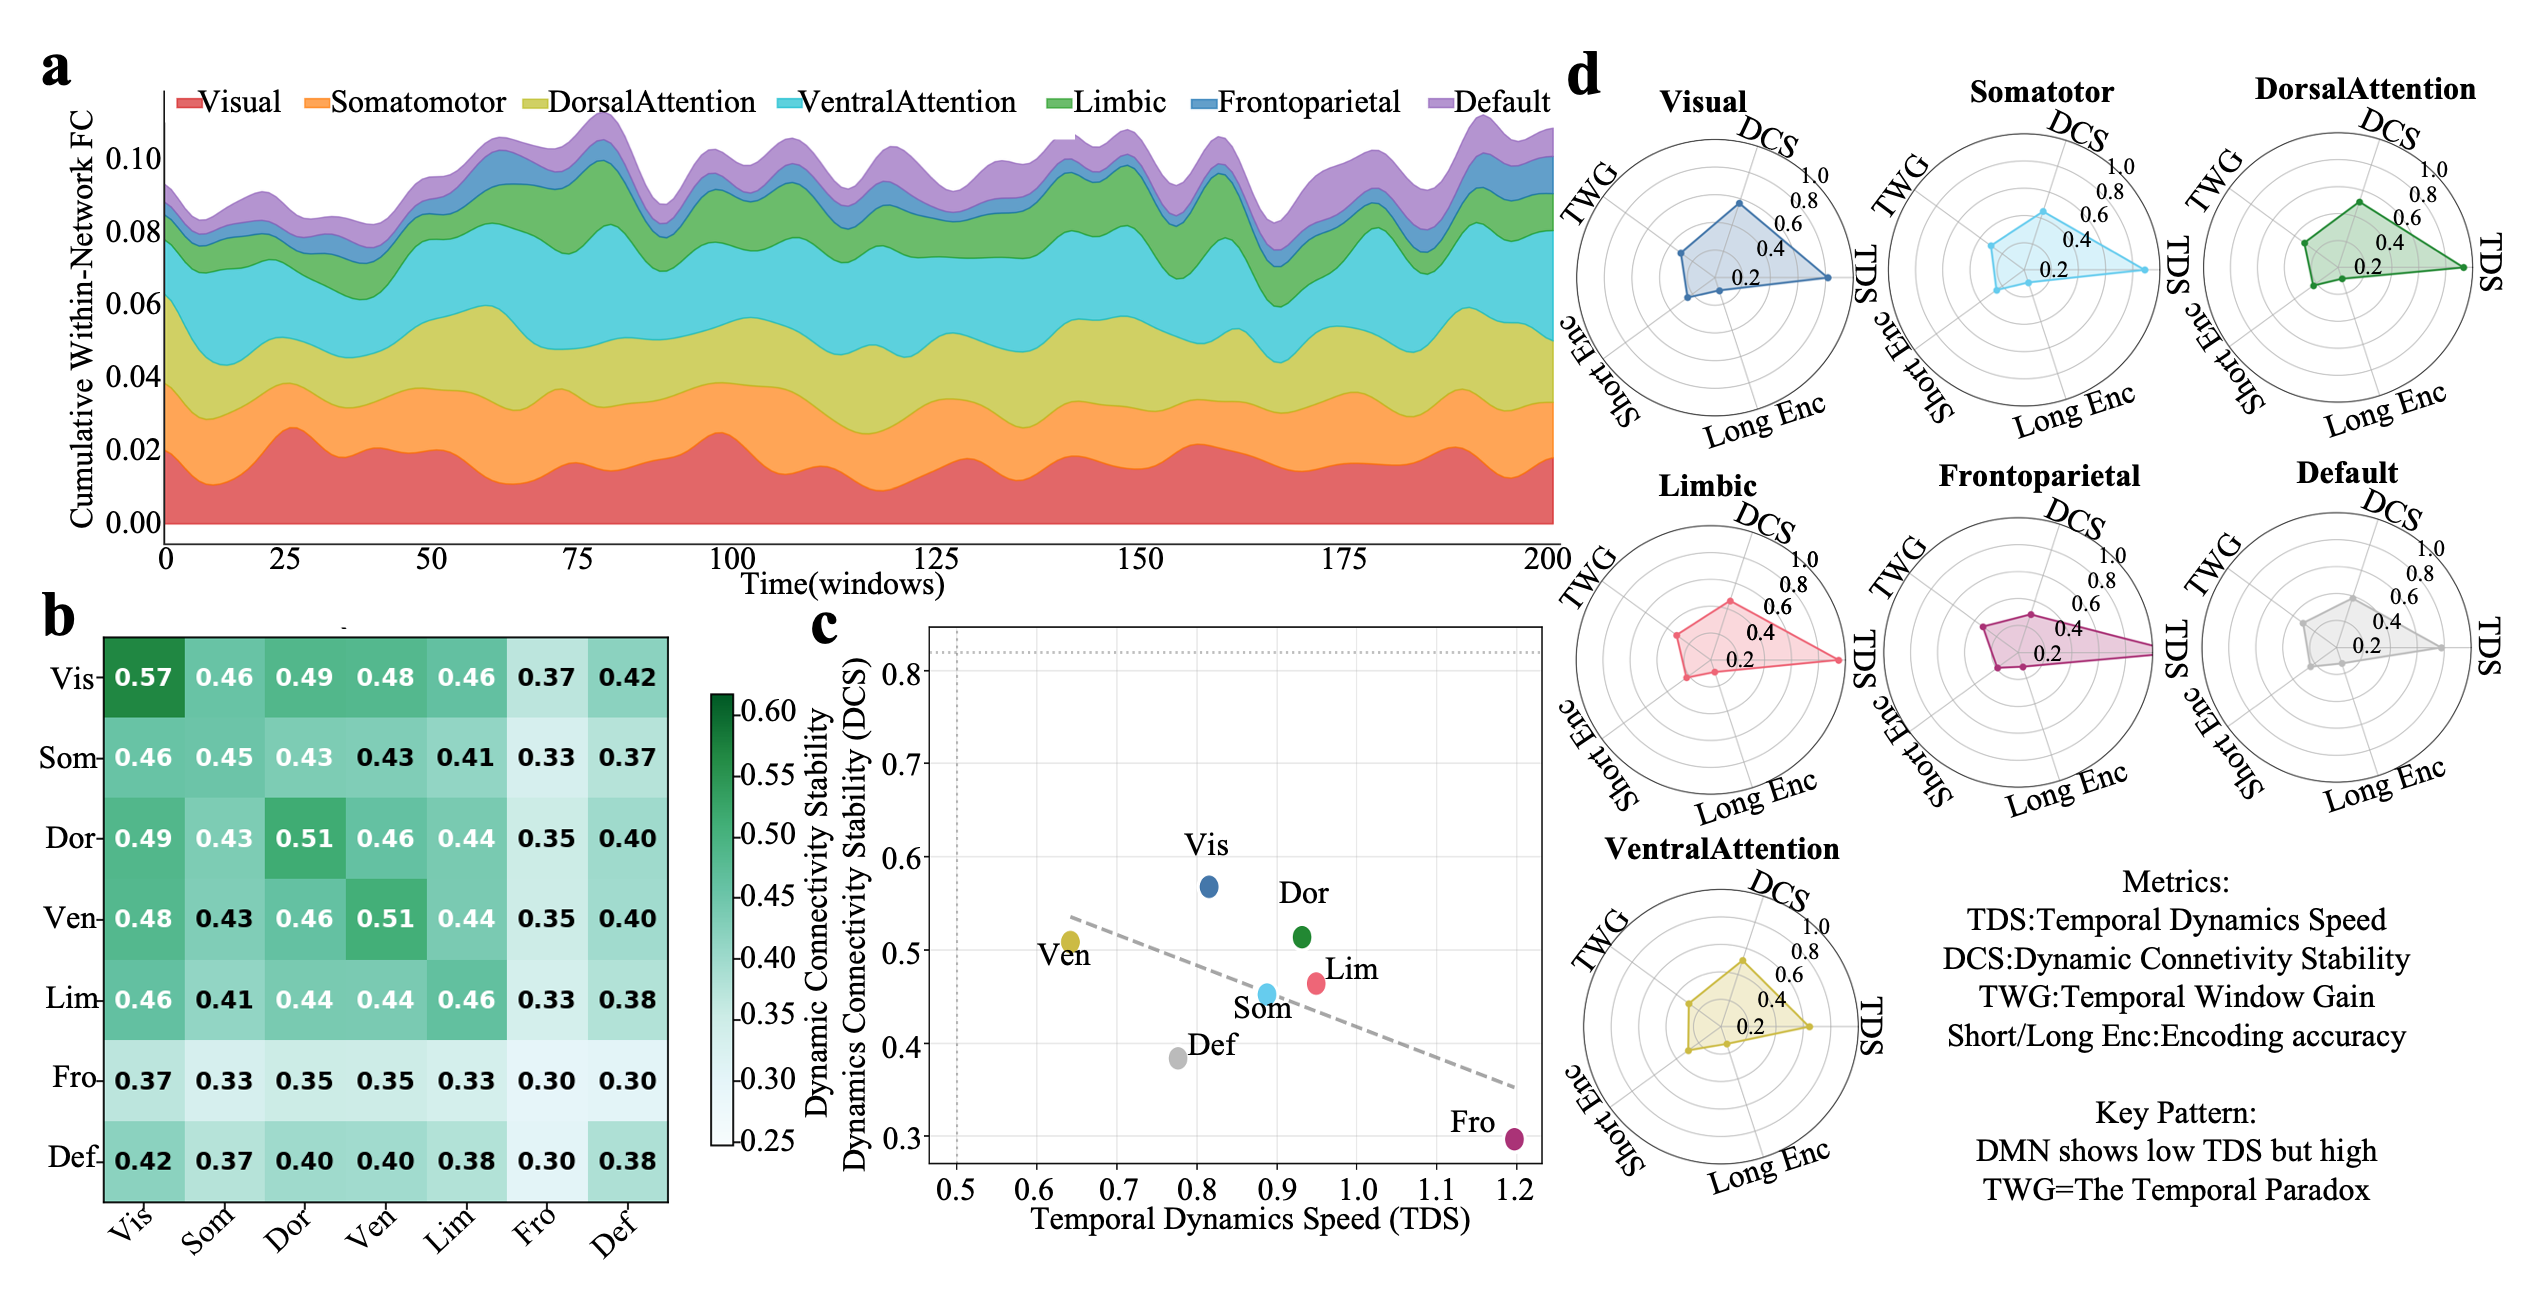
\includegraphics[width=0.95\textwidth]{figures/fig03_dcs_radar.png}
    \caption{\textbf{Dynamic Connectivity Stability and Network Profiles.} (a) Stream graph of cumulative within-network functional connectivity (mean pairwise Pearson $r$ within each network) over time; data from a representative participant (sub-01) viewing \textit{Friends}, showing first 200 windows ($\sim$50 min). (b) Inter-network DCS stability matrix. (c) TDS vs DCS scatter plot; dashed line shows non-significant correlation ($r = -0.32$, $p = .48$). (d) Radar charts of network profiles integrating TDS, DCS, TWG, and encoding accuracy.}
    \label{fig:dcs_radar}
\end{figure*}
Beyond temporal dynamics speed, we examined functional connectivity stability (Figure~\ref{fig:dcs_radar}a shows representative single-subject data). Connectivity fluctuations differed across networks (Kruskal-Wallis $H = 45.3$, $p < .001$). Visual Network showed the highest stability (DCS $= 0.57$), while Frontoparietal showed the lowest (DCS $= 0.30$; Figure~\ref{fig:dcs_radar}b; see Table~\ref{tab:network_summary}). The correlation between TDS and DCS was non-significant ($r = -0.32$, $p = .48$; Figure~\ref{fig:dcs_radar}c), suggesting connectivity stability reflects a distinct dimension of network organization.

\subsection{Integrated Network Profiles}

Table~\ref{tab:network_summary} summarizes temporal metrics and encoding performance. Radar charts (Figure~\ref{fig:dcs_radar}d) reveal distinct network profiles: fast networks show high TDS but variable connectivity stability; slow networks show low TDS with higher stability. The anatomical distribution (Figure~\ref{fig:brain_glass}) shows fast processing regions concentrated in frontoparietal cortices, while slow regions distribute across ventral attention and default mode areas. Network TDS rankings (Figure~\ref{fig:tds_ranking}) range from Frontoparietal (TDS $\approx 1.2$) to Ventral Attention (TDS $\approx 0.64$).


\begin{table}[htbp]
\centering
\small
\setlength{\tabcolsep}{3.5pt}
\caption{\textbf{Summary of Network Temporal Properties and Encoding Performance}}
\label{tab:network_summary}
\begin{tabular}{lcccccc}
\toprule
\textbf{\shortstack[t]{Network\\~}} & \textbf{\shortstack[t]{TDS\\~}} & \textbf{\shortstack[t]{DCS\\~}} & \textbf{\shortstack[t]{TWG\\~}} & \textbf{\shortstack[t]{Ridge\\$r$}} & \textbf{\shortstack[t]{LSTM\\$r$}} & \textbf{\shortstack[t]{LSTM\\Gain}} \\
\midrule
Frontoparietal    & 1.20 & 0.30 & $-0.015$ & 0.277 & 0.408 & +47.5\% \\
Limbic            & 0.95 & 0.46 & $-0.024$ & 0.305 & 0.456 & +49.3\% \\
Dorsal Attention  & 0.93 & 0.51 & $-0.026$ & 0.285 & 0.425 & +49.5\% \\
Somatomotor       & 0.89 & 0.45 & $-0.029$ & 0.327 & 0.514 & +57.4\% \\
Visual            & 0.82 & 0.57 & $-0.028$ & 0.317 & 0.492 & +55.4\% \\
Default           & 0.78 & 0.38 & $-0.021$ & 0.386 & 0.582 & +50.8\% \\
Ventral Attention & 0.64 & 0.51 & $-0.029$ & 0.423 & 0.632 & +49.3\% \\
\bottomrule
    \end{tabular}
\begin{tablenotes}
\footnotesize
\item \textit{Note.} TDS = Temporal Dynamics Speed; DCS = Dynamic Connectivity Stability; TWG = Temporal Window Gain (ridge regression, long [25 TRs] minus instant [1 TR] window); Ridge/LSTM $r$ = encoding accuracy (sequence length = 20 TRs); LSTM Gain = percentage improvement over ridge. Networks sorted by TDS (fastest to slowest).
\end{tablenotes}
\end{table}




%% ============================================================
%% SECTION 4: DISCUSSION
%% ============================================================

\section{Discussion}

\subsection{Summary of Findings}

This study investigated cortical temporal dynamics during naturalistic movie viewing, yielding three main findings. First, functional networks differ systematically in temporal dynamics speed (RQ1). Second, our hypothesis that slower networks would benefit more from temporal integration was not supported: all networks showed negative TWG, and TDS did not predict integration benefit. However, LSTM models that preserve temporal structure improved encoding by 47--57\% uniformly across all networks, resolving the paradox: temporal integration benefits neural encoding universally, but only when temporal dependencies are properly modeled. Third, connectivity stability represents a distinct dimension of network organization, uncorrelated with TDS.

\begin{figure}[!t]
    \centering
    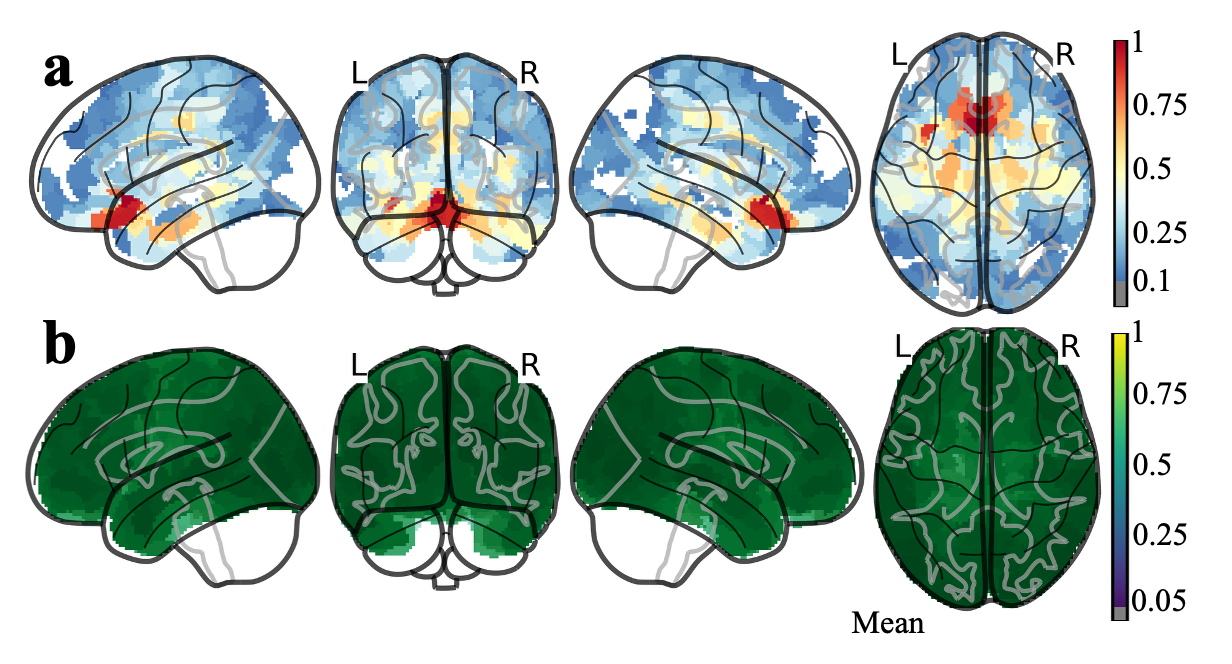
\includegraphics[width=0.45\textwidth]{figures/fig08_brain_glass_overview.png}
    \caption{\textbf{Brain Glass Visualization of Temporal Dynamics.} (a) Temporal Dynamics Speed (TDS) across cortex: fast (red/warm) vs slow (blue/cool). (b) Network Temporal Hierarchy, color-coded by network position in temporal gradient.}
    \label{fig:brain_glass}
\end{figure}

The temporal hierarchy we observed diverges from canonical descriptions. Previous work suggested a simple unimodal-to-transmodal gradient \citep{murray2014hierarchy, hasson2008hierarchy}. Our spectral-based TDS metric reveals more nuanced organization: Frontoparietal Network exhibited the fastest dynamics, aligning with its role in rapid cognitive control \citep{badre2018frontal}; Ventral Attention showed the slowest, consistent with sustained attention functions; Default Mode exhibited intermediate dynamics, supporting reconceptualizations of DMN as dynamically flexible \citep{gao2020neuronal}. Importantly, connectivity stability (DCS) was uncorrelated with TDS, indicating that fast networks can have either stable or variable connectivity patterns. For example, the Visual Network combines moderate TDS with high stability, while Frontoparietal shows fast dynamics but low stability. This multi-dimensional view suggests networks are characterized by independent temporal properties rather than a single speed gradient.

\begin{figure}[!t]
    \centering
    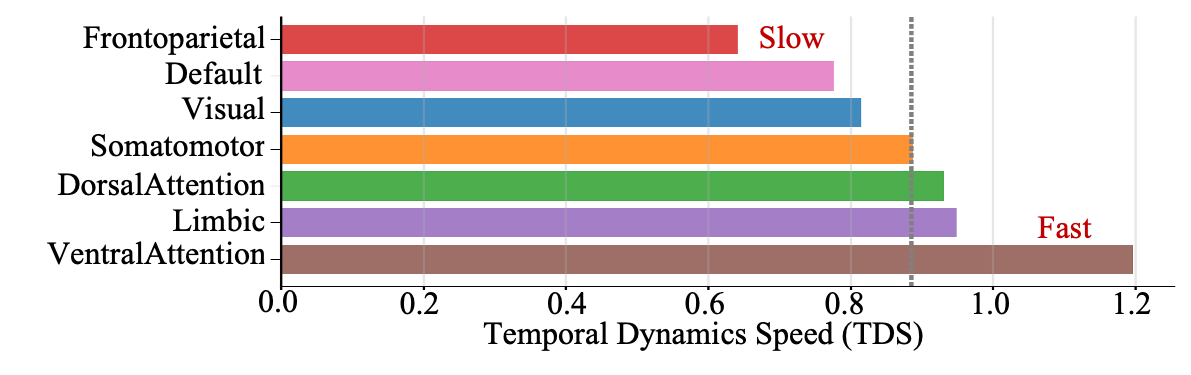
\includegraphics[width=0.48\textwidth]{figures/fig09.png}
    \caption{\textbf{Network TDS Ranking.} Temporal Dynamics Speed (TDS) for each functional network, ordered from slowest (Ventral Attention, TDS $= 0.64$) to fastest (Frontoparietal, TDS $= 1.20$). Dashed vertical line indicates TDS $= 1.0$, separating networks with predominantly slow dynamics (TDS $< 1$) from those with fast dynamics (TDS $> 1$). Only Frontoparietal Network exceeds this threshold, indicating predominantly high-frequency activity.}
    \label{fig:tds_ranking}
\end{figure}

\subsection{The Temporal Integration Paradox Resolved}

Simple temporal averaging impaired encoding accuracy, appearing to contradict temporal integration benefits. The LSTM comparison resolves this paradox: the problem lies not with temporal integration itself, but with implementation. Simple averaging destroys temporal structure, while recurrent architectures preserve sequential dependencies. This ``structured temporal integration'' view aligns with recurrent processing mechanisms \citep{honey2012slow} and hierarchical predictive coding \citep{kiebel2008hierarchy}, reconciling our findings with prior work proposing that slow dynamics support deep comprehension \citep{hasson2015hierarchical}.

What do these findings imply for our understanding of cortical temporal organization? The uniform LSTM benefit across all networks, regardless of intrinsic dynamics speed, indicates that temporal structure is universally important for neural encoding. This challenges the prediction that slow networks should benefit more; instead, all networks exploit temporal dependencies, suggesting naturalistic stimuli contain temporal structure at multiple scales that all networks must process. This finding aligns with recent advances in deep learning-based brain encoding, which have demonstrated that recurrent architectures capturing temporal dependencies substantially outperform static models \citep{oota2024deep}. From a practical standpoint, encoding models should preserve temporal dependencies rather than aggregate features across time.

\subsection{Limitations}

Several limitations should be noted: (1) four participants limits generalizability despite intensive within-subject sampling; (2) our TDS metric differs from traditional approaches, potentially explaining divergent network orderings; (3) negative TWG could reflect factors beyond averaging (e.g., HRF modeling limitations); (4) network-level analysis may obscure region-level heterogeneity. Future work should compare TDS with autocorrelation-based metrics and explore alternative temporal aggregation methods.


%% ============================================================
%% SECTION 5: CONCLUSIONS
%% ============================================================

\section{Conclusions}

This study investigated cortical temporal dynamics during naturalistic movie viewing. Functional networks exhibit a clear temporal hierarchy (RQ1), but our hypothesis that slower networks would benefit more from temporal integration was not supported (RQ2): all networks showed impaired encoding with temporal averaging, yet all benefited equally from LSTM models (+47--57\%). These findings resolve an apparent paradox: temporal integration benefits neural encoding universally, but only when temporal structure is preserved rather than averaged. For computational neuroscience, encoding models should preserve temporal dependencies; the $\sim$50\% LSTM improvement demonstrates that temporal structure accounts for substantial neural response variance during naturalistic viewing.

% \section{Acknowledgments}

% In accordance with conference guidelines, we disclose AI tool usage: Claude (Anthropic) was used to assist with code development for data analysis pipelines and manuscript editing. All scientific interpretations, experimental design decisions, and conclusions were made by the human authors. Data were obtained from the Algonauts 2025 Challenge (CNeuroMod dataset).

\printbibliography

\end{document}
